%% ═══════════════════════════════════════════════════════════════════════════
\subsection{Introduction and Key Definitions}
\label{sec:lit_intro}
%% ═══════════════════════════════════════════════════════════════════════════

This review answers a single question: which existing methods can be assembled to measure,
correct and propagate a biased urgency signal, and which part of that assembly is missing from
the literature? The relevant work is broad but fragmented across operations research,
behavioural science and digital twin engineering, and read individually each stream solves one
piece. Read together they leave a specific slot empty: no retrieved work combines, within a
single supply chain decision architecture, a multi-block operational urgency function, a
structured client-side urgency input, an adequacy layer comparing stated and operational
urgency, network propagation across a multi-tier DAG, and empirical validation of the adequacy
signal against recorded
outcomes~\autocite{sawik2013integrated,sawik2014joint,sawik2016integrated,cohen2021assigning,hosseini2020bayesian}.
The review is organised by the role each stream plays in that argument rather than by
chronology, 

Six terms carry specific meanings throughout. \textbf{Urgency} is how far a task needs prompt
action to avoid a material loss of operational performance; \emph{importance} is about
strategic value and \emph{priority} about current execution order, and a task can be important
and not urgent, or first in the queue for reasons connected to
neither~\autocite{cheng2025survey,zhu2018mere}. \textbf{Real-time scheduling} covers algorithms
assigning execution order under temporal and resource
constraints~\autocite{pinedo2012scheduling}, drawn on here only as historical grounding for
deadline-sensitive value functions, since no scheduling algorithm is delivered. A
\textbf{digital twin} is a synchronised digital representation of a physical system supporting
monitoring, simulation and decision-making from real-time and historical
data~\autocite{ivanov2020digital}. \textbf{\Gls{mcdm}} covers
methods combining potentially conflicting performance dimensions into a single
decision~\autocite{saaty1980analytic,brans1986promethee}. The \textbf{\Gls{pi}} is the model of open, mutualised logistics networks routing shipments through
shared infrastructure in standardised modular containers~\autocite{montreuil2011toward}. And a
\textbf{serious game} is a simulation environment designed to train decision-makers through
realistic scenarios with immediate feedback and
scoring~\autocite{sterman1989modeling,prensky2001digital}.

%% ═══════════════════════════════════════════════════════════════════════════
\subsection{Risk Propagation and Deadline-Sensitive Value}
\label{sec:lit_temporal}
%% ═══════════════════════════════════════════════════════════════════════════

Within real-time systems, deadline-sensitive scheduling theory models task value as a
function of completion or response time, an approach known as time-value or utility-accrual
scheduling~\autocite{cheng1996due,cheng2025survey}. Chen and
M\"uhlethaler~\autocite{cheng1996due} show that task utility is typically constant up to a
deadline and then non-increasing with delay, and a broader survey confirms that
deadline-sensitive literature models task value as a function of response time with
bounded, structured degradation after critical thresholds~\autocite{cheng2025survey}. This
establishes the precedent for treating urgency as time-varying, but it stops at a single
task in isolation.

A complementary line of evidence comes from network risk propagation. Ivanov and colleagues
formalise the ripple effect, whereby a local disruption at one supplier cascades through
downstream tiers and amplifies as it
travels~\autocite{ivanov2020digital,ivanov2019viable,li2020exploring}. Probabilistic risk
inference for supply chain systems~\autocite{Zhe20} further shows that aggregating
heterogeneous risk indicators into a single node-level score is itself an open modelling
question, distinct from how that score should then be propagated.

Table~\ref{tab:urgency_models} compares four candidate aggregation and growth models found
across these two lines, and Figure~\ref{fig:aggregation_families} plots what each one does.

\begin{figure}[htbp]
    \centering
    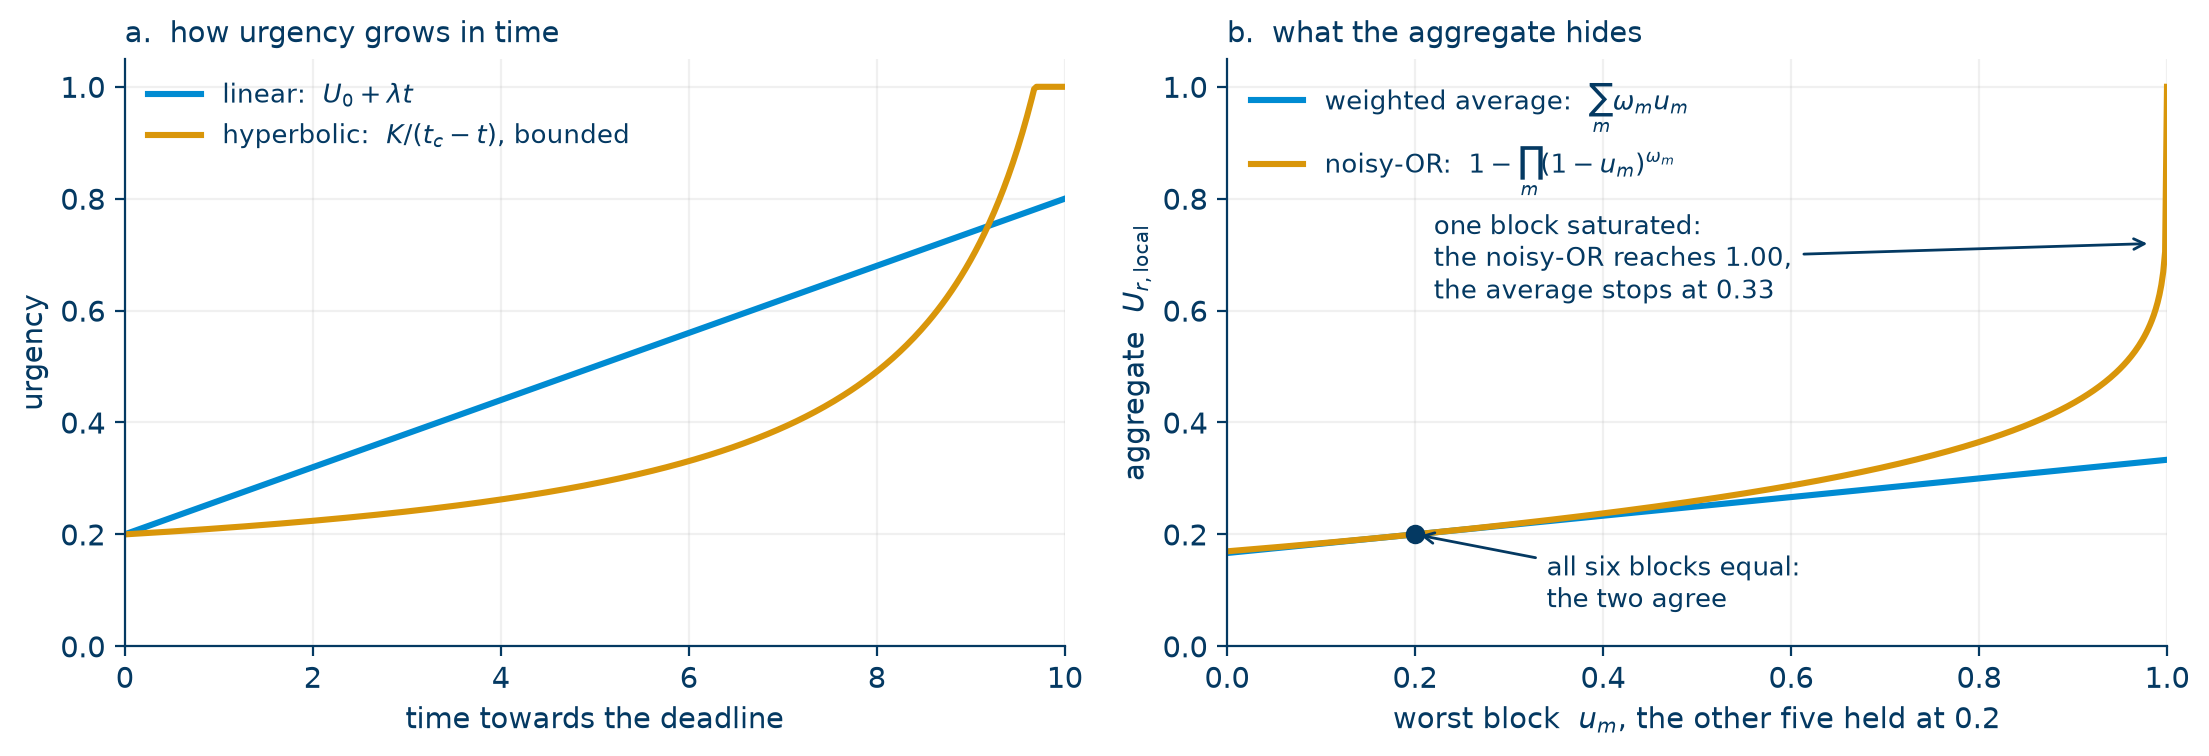
\includegraphics[width=\linewidth]{Images/aggregation_families.png}
    \caption[The four candidate models, plotted]{The four models of
    Table~\ref{tab:urgency_models}. Panel~b is the choice this thesis has to make: a weighted
    average is fully compensatory, so a catastrophic reading on one block is offset by
    acceptable readings elsewhere and the aggregate stops at $0.33$; a noisy-OR is not, and
    any factor approaching its maximum drives the aggregate towards its own maximum whatever
    the others read. Which behaviour is desirable depends on whether the aggregate describes
    average condition or exposure to the worst active cause, and the composite-indicator
    literature treats that as a modelling decision rather than a solved
    question~\autocite{greco2018,becker2017}.}
    \label{fig:aggregation_families}
\end{figure}

The hyperbolic family carries a further caveat. A structurally similar acceleration appears
in \gls{lppl} models of financial crash
precursors~\autocite{johansen2001finite,johansen2000crashes}, but empirical analyses find
LPPL-family models highly parameter-sensitive and unsuited to use as production risk
models~\autocite{feigenbaum2001statistical,bree2010prediction}.

\paragraph{Gaps in risk propagation and deadline-sensitive value.}
Neither stream specifies how to aggregate heterogeneous, block-structured operational risk
indicators at a single node before propagating them. Neither addresses declared urgency, or
the mismatch between what is stated and what is computable. And the aggregation literature
stops at the observation that the choice matters, without establishing whether equal values
on structurally different indicators carry equal risk meaning, which is the question any
multi-block aggregate has to answer before it can be interpreted.

%% ═══════════════════════════════════════════════════════════════════════════
\subsection{Cognitive Bias in Urgency Declaration}
\label{sec:lit_bias}
%% ═══════════════════════════════════════════════════════════════════════════

Human decision-makers systematically misrepresent urgency. Two lines of behavioural
operations research establish it from different angles, and both bear directly on any
system that takes operator-declared urgency as an input.

\textcite{zhu2018mere} report the Mere-Urgency Effect in five controlled experiments:
participants consistently over-prioritised imminent low-value tasks over distant
high-value tasks, and the bias persisted even when participants were informed of its
existence. \textcite{steel2006integrating} provides a complementary formal model
through the \gls{tmt}:

\begin{equation}
    V(t) = \frac{U \times E}{1 + \Gamma \times D(t)^k},
    \label{eq:tmt_val}
\end{equation}

where $U$ is objective utility, $E$ is the expectancy of success, $D(t)$ is the delay to
deadline, and $\Gamma$ and $k$ are individual discounting parameters. As the delay to
deadline shrinks towards zero, the motivational value $V(t)$ converges to the full product
of utility and expectancy, so immediacy becomes more salient as the deadline approaches.
Near-term tasks can therefore attract disproportionate attention even when their broader
objective value is lower~\autocite{steel2006integrating}.
Table~\ref{tab:tmt_vars} gives the operational role of each parameter.

These laboratory findings are supported by evidence from operational settings. \textcite{rusou2020psychology} show that operators under workload preferentially
complete small, easy tasks, the operational analogue of under-triage for large-scope supply
chain activities. \textcite{diwa2020task} confirm in a large field study
that completing easy tasks first significantly hurts overall performance. Hospital
admission control under occupancy uncertainty~\autocite{kim2020admission} produces over-
and under-triage patterns analogous to those seen in logistics operators facing uncertain
lead times. Human-centred decision support systems such as that of \textcite{rosenthal2020human} use visual feedback to show the mismatch between human
plans and system temporal constraints, helping users calibrate their schedules.

\paragraph{Gaps in cognitive bias research.}
Behavioural research diagnoses the problem and quantifies it in controlled settings, but
the magnitude of the bias in industrial supply chain contexts remains a matter of
calibration, and this literature does not prescribe a real-time operational correction.

%% ═══════════════════════════════════════════════════════════════════════════
\subsection{Indicators of Delivery Rupture Risk}
\label{sec:lit_indicators}
%% ═══════════════════════════════════════════════════════════════════════════

If urgency is to be aggregated from several indicators, the literature has to supply the
indicators. This section reviews the body of work that identifies which observable
quantities precede a delivery rupture, meaning a failure to deliver at the agreed time,
place, quantity and quality. It is the source from which
Section~\ref{sec:model_blocks} later selects.

Heckmann, Comes and Nickel establish rupture as the terminal event a supply risk measure
should anticipate, and criticise the field for measuring exposure without connecting it to
that event~\autocite{heckmann2015critical}. Indicator-based supplier monitoring proceeds by
identifying observable precursors rather than modelling the event
directly~\autocite{mokhtar2019supplier}.

Table~\ref{tab:precursors} gives the five families of precursor that recur across that work,
with the sources establishing each and the reason it is a precursor rather than a symptom.
Section~\ref{sec:model_blocks} selects from this table, and Section~\ref{sec:model_blocks} states what it kept.

\paragraph{Gap in the indicator literature.}
The families are named individually and no retrieved work supplies a criterion for deciding
which of them belong in one composite, nor a rule for combining them once chosen. That is the
question Section~\ref{sec:model_ur} answers with an explicit independence assumption rather
than with a weighting convention.

\subsection{Closest Antecedents: Network Risk Twins and MCDM Supplier Scoring}
\label{sec:lit_antecedents}
%% ═══════════════════════════════════════════════════════════════════════════

The works most structurally similar to this thesis combine multi-criteria supplier scoring
with disruption-aware network monitoring.
\textcite{sawik2013integrated} develops mixed-integer programming models for resilient
supplier order assignment integrating cost, service level and disruption risk, extended in
later work to joint and integrated
formulations~\autocite{sawik2014joint,sawik2016integrated}. \textcite{cohen2021assigning} and \textcite{afrasiabi2022extended}
extend this to \gls{mcdm} supplier prioritisation under disruption, combining criteria
weighting with allocation optimisation. \textcite{chakrabortty2020efficient} confirm that rule-based heuristics remain
competitive against exact methods in dynamic industrial environments. These works are cited
for the closeness of their subject matter, not because this thesis reuses their
optimisation machinery, which addresses allocation and sequencing rather than urgency
measurement.

\paragraph{Gaps in the closest antecedents.}
Two gaps distinguish this stream from the present work. First, none introduces a
network-propagated urgency signal computed independently at every node and combined across
tiers; risk is typically evaluated once, at the point of decision. Second, none compares a
client-stated urgency against a model-derived urgency: where the declared signal exists at
all, it is used directly, without validation against live operational proxies.

%% ═══════════════════════════════════════════════════════════════════════════
\subsection{Enabling Method: Bayesian and Probabilistic Risk Updating}
\label{sec:lit_bayes}
%% ═══════════════════════════════════════════════════════════════════════════

Bayesian methods are a well-supported approach for revising risk estimates from new
evidence in supply chain
research~\autocite{pearl1988probabilistic,koller2009probabilistic}. Rather than a full
Bayesian network with an explicit conditional-probability-table structure, this study draws
on the narrower and more tractable case of Beta-Bernoulli conjugate updating: a failure
probability $p$ is treated as a Beta-distributed belief with an equivalent prior sample
size $n_0$, revised from a small number of newly observed equivalent trials $(k, n)$ each
time a calibrated operational event is declared.

Three convergent findings support this choice. \textcite{hosseini2020bayesian} survey Bayesian methods applied to supply chain risk
and resilience, finding that probabilistic belief-revision methods are often preferred to
deterministic scoring when sparse new evidence must update an existing estimate. \textcite{huang2020bayesian} and \textcite{deng2020prediction}
develop Bayesian models for disruption and delay probability estimation.
\textcite{lockamy2011bayesian} and \textcite{qazi2017dynamic} support
Bayesian revision as a practical tool under sparse, event-driven evidence, consistent with
the small-sample setting of a weekly-cadence digital twin. Plain frequency counts, by
contrast, are unstable when only a handful of events are declared per node per
project~\autocite{zheng2020risk}.

\paragraph{Gaps in Bayesian risk updating.}
Bayesian belief revision quantifies disruption exposure but does not, by itself, compare it
against a client-declared urgency, and it says nothing about whether the resulting
probabilities are well calibrated once they reach a human reader.

%% ═══════════════════════════════════════════════════════════════════════════
\subsection{Enabling Method: Digital Twins and Real-Time Decision Support}
\label{sec:lit_dt}
%% ═══════════════════════════════════════════════════════════════════════════

The digital twin concept was formalised by \textcite{grieves2014digital} as a
virtualised representation of a physical process. \textcite{tao2018digital}
extended it to manufacturing, and \textcite{fuller2020digital} surveyed the
enabling technologies. In supply chain management, \textcite{ivanov2021digital} define the \gls{sc} \gls{dt} as integrating simulation,
optimisation and machine learning. \textcite{ivanov2020digital} address
digital supply chain twins for disruption risk and resilience management. \textcite{wang2020digital} demonstrate twin-driven planning in a manufacturing context
analogous to DISCO's satellite component network. In the Industry~5.0 setting, these
systems have evolved towards human-in-the-loop Cognitive Digital Twins, where semantic
models and reasoning methods capture human feedback and synchronise mental models with
simulated physical operations~\autocite{niloofar2023}.

Real-time freight planning work shows that operational urgency proxies, meaning slack,
lateness risk and shortage exposure, are already present within these
systems~\autocite{hrusovsky2021realtime,perez2022digital}. Model-predictive control for
vehicle routing~\autocite{karam2022realtime} and twin-based disruption
response~\autocite{ding2023realtime,leung2022digital,zhu2025industry5} confirm the state of
the art in live operational replanning.

\paragraph{Gaps in digital twin decision support.}
In the retrieved literature, no system combines a declared urgency input, a computed
operational urgency, and their propagated mismatch within one architecture. A second gap
matters for this thesis specifically: these systems are evaluated on the accuracy of their
physical state estimation, and their inputs are assumed to arrive. Where an input depends
on the same operator whose judgement the system exists to support, that circularity is not
usually treated as a measurement problem.

%% ═══════════════════════════════════════════════════════════════════════════
\subsection{Enabling Methods: Multi-Criteria Decision Methods}
\label{sec:lit_mcdm}
%% ═══════════════════════════════════════════════════════════════════════════

This research builds on two distinct domains within multi-criteria decision-making:
pairwise comparison methods for eliciting weights, and outranking aggregation for turning
those weights into a defensible ranking of nodes.

Table~\ref{tab:mcdm} compares the four methods on the three axes that decide which is usable
here: what an elicitation costs the operator, what the method returns, and whether a good
score on one criterion can hide a bad score on another.

The last column of that table is why both an elicitation method and an outranking method are
used rather than one. Weighted averages are fully compensatory: an excellent score on one
criterion masks a critical failure on another. Outranking builds pairwise preference flows
instead, which prevents that masking, and a cross-industry survey confirms its suitability for
supplier and node evaluation. Composite-index work nonetheless warns that nominal weights
often diverge from effective importance through correlation, normalisation and aggregation
dynamics, and that the choice of normalisation is itself non-neutral because it can produce
rank reversal~\autocite{greco2018,becker2017,triantaphyllou2000multi}.

\paragraph{Gaps in multi-criteria decision methods.}
These methods weight criteria and rank alternatives, and they are static elicitation and
aggregation tools. None is routinely compared against a computed operational counterpart. And
the composite-indicator critique is generally raised as a caveat at the end of a paper rather
than turned into something a running system can check on its own data.

\subsection{Forecast-Assisted Decision and Automation Bias}
\label{sec:lit_automation}
%% ═══════════════════════════════════════════════════════════════════════════

The streams above concern how to compute a signal. This one concerns what happens when the
signal is shown to the person whose judgement it was built to support, and it is included
because the campaign reported in Section~\ref{sec:res_armB} produced a result in exactly
that register.

\textcite{parasuraman1997humans} set out the canonical taxonomy of
misuse, disuse and abuse of automation, establishing that the failure modes of automated
aids are as much about human reliance as about machine accuracy. \textcite{skitka1999automation} demonstrate automation bias directly: participants
supported by an automated aid committed both omission errors, failing to react to a problem
the aid did not flag, and commission errors, following the aid against contradicting
evidence. \textcite{cummings2004automation} extends the finding to time-critical
decision support, the family to which a weekly supply chain review belongs. \textcite{goddard2012automation} provide a systematic review in clinical
decision support, and report that automation bias is frequent, that it is mediated by the
confidence with which advice is presented, and that it is only partially mitigated by
training.

The direction of the effect is not uniform. \textcite{dietvorst2015algorithm} document algorithm aversion, where people abandon
an algorithm after seeing it err even when it outperforms them, while
\textcite{logg2019algorithm} document algorithm appreciation, where
people weight algorithmic advice more heavily than human advice. \textcite{bansal2021whole} show that adding explanations to a model's output can
increase acceptance of its recommendations whether or not those recommendations are
correct, so that explanation improves persuasion more reliably than it improves joint
accuracy.

Two consequences follow for the present work. First, an advisory signal changes the
behaviour it measures, which means a system that both elicits declared urgency and displays
a forecast to the declarant is not observing an independent signal. Second, a confidently
presented but poorly calibrated probability is a specific hazard rather than a cosmetic
defect, since the confidence with which advice is presented is itself a mediator of
reliance~\autocite{goddard2012automation}.

\paragraph{Gaps in forecast-assisted decision research.}
This literature is dominated by single-decision laboratory tasks and clinical decision
support. It does not address a repeated, multi-turn setting in which the same operator is
shown a forecast about their own node, week after week, while their declaration feeds back
into the model's state. Nor does it address the case where the displayed forecast is
systematically miscalibrated in a known direction, which is the situation measured in
Section~\ref{sec:res_armA_scored}.

%% ═══════════════════════════════════════════════════════════════════════════
\subsection{Validation Methodology: Serious Games}
\label{sec:lit_games}
%% ═══════════════════════════════════════════════════════════════════════════

The Beer Game~\autocite{sterman1989modeling} is the foundational supply chain serious game.
Sterman shows that players systematically misperceive the feedback in their own supply
line, underestimating orders already placed but not yet received, and over-order with a lag
once a shortage appears, amplifying the resulting oscillation as it travels upstream, the
mechanism known as the bullwhip effect~\autocite{lee1997bullwhip}. This decision bias is
analogous to the false-urgency pathology, where an operator over-reacts to a signal after a
delay rather than adjusting smoothly. \textcite{prensky2001digital} establishes the
theoretical basis for digital game-based learning, and \textcite{deterding2011game} formalise gamification design principles.

\textcite{mohaddesi2020gamettes} introduce the Gamette methodology, a
bite-sized approach to capturing decision-making patterns for behavioural modelling,
directly applicable to a weekly-review protocol in which operators repeatedly submit
urgency assessments. \textcite{bellotti2013framework} provide an evaluation
framework for serious game learning outcomes. \textcite{lafkihi2025freight} use a freight transportation game to study carrier
behaviour on online spot-market platforms, a setting connected to the Physical Internet's
vision of mutualised capacity allocation.

\paragraph{Gaps in serious game validation.}
Serious games are established as instruments for observing decision bias, but they are
usually scored on learning outcomes or on aggregate system performance. They are rarely
used as a controlled comparison in which the same frozen scenario is replayed with and
without a treatment applied to the declarant, which is the design adopted in
Section~\ref{sec:methods_arms}.

%% ═══════════════════════════════════════════════════════════════════════════
\subsection{Probabilistic Forecast Verification}
\label{sec:lit_verification}
%% ═══════════════════════════════════════════════════════════════════════════

Because this thesis scores a probabilistic forecast against recorded outcomes, it inherits
the vocabulary of forecast verification. \textcite{brier1950verification} introduced
the mean squared error of probabilistic forecasts, and
\textcite{murphy1973vector} decomposed it into reliability, resolution and
uncertainty, establishing the distinction this thesis relies on: a forecast can order
outcomes correctly while announcing the wrong probabilities, and the two failures require
different remedies. \textcite{gneiting2007strictly} formalise strictly
proper scoring rules, under which a forecaster minimises expected loss only by reporting
their true belief.

The distinction has been rediscovered in machine learning. \textcite{niculescu2005predicting} show that several strong classifiers produce
distorted probabilities that require post-hoc correction, and \textcite{guo2017calibration} show that modern neural networks are systematically
over-confident, with accuracy improving while calibration degrades. Both report that the
correction is a separate, cheap, post-hoc layer rather than a change to the model.

\paragraph{Gaps in forecast verification practice.}
The verification literature assumes the outcome being predicted is unambiguously defined.
In an operational supply chain setting it is not: whether a node-week counts as an adverse
outcome depends on choices about which events qualify and over what horizon.
Section~\ref{sec:res_target_trap} shows that this choice, and nothing else, moves the
measured skill of the same forecasts by a factor of five.

%% ═══════════════════════════════════════════════════════════════════════════

\subsection{Analogical and Contextual Literature}
\label{sec:lit_analogy}
%% ═══════════════════════════════════════════════════════════════════════════

Three streams provide vocabulary and context rather than foundations, and are flagged as
non-foundational wherever they are used.

\paragraph{Medical triage as a conceptual analogy.}
Medical triage provides an analogy for prioritising under severe capacity constraints and
cognitive pressure. Protocols such as the \gls{mts}~\autocite{mackway2013emergency} categorise patients into five urgency levels
using flowcharts, whereas the Emergency Severity Index integrates predicted resource
consumption. Comparative clinical studies show substantial classification discrepancies between the two
systems, at a weighted $\kappa = 0.51$, so even trained professionals disagree on urgency
assessment~\autocite{kuligowski2025comparative}. The clinical literature also establishes an
asymmetry that logistics work rarely states explicitly: under-triage, meaning a patient
classified as less urgent than they are, is more dangerous than over-triage, because the
first costs a life and the second costs a
queue~\autocite{kim2020admission,mackway2013emergency}.

\paragraph{Physical Internet and synchromodality.}
The Physical Internet is a model of interconnected logistics networks in which routing,
storage and transport assets are mutualised across actors~\autocite{montreuil2011toward}. In
such networks urgency stops being a local concern and becomes a network-level quality of
service variable, because the capacity one actor claims is capacity another loses.

A related but separate concept is synchromodality. Where the Physical Internet describes who
shares the infrastructure, synchromodality describes when the mode is chosen: a shipment can
be moved between road, rail and waterway in real time as conditions change, instead of
being committed to one mode when it is booked. The two can operate together and neither
presupposes the other. Dynamic routing under synchromodality needs priority signals that
stay valid across rolling planning windows~\autocite{guo2020dynamic}, and disruptions travel
quickly through interconnected networks, producing cascading ripple
effects~\autocite{li2020exploring}.

\paragraph{Regulatory carbon accounting.}
Corporate sustainability reporting requirements have made transport emissions a reported
quantity rather than an optional one~\autocite{cordova2024green}. The \gls{glec} Framework
v3.2~\autocite{smartfreight2023glec} and \gls{vecto}~\autocite{commission2017vecto} define
emissions baselines for heavy goods vehicles, and emissions factors relate non-linearly to
vehicle speed and cargo load, so a carbon figure cannot be recovered from cost or distance
alone~\autocite{ademe2014impacts}.

\paragraph{Earth observation of built and logistics assets.}
The opening reported in Section~\ref{sec:res_volume} rests on a separate literature.
Overhead object detection has a standard benchmark in DOTA~\autocite{xia2018dota}, whose
oriented bounding boxes and vehicle classes make it the reference for overhead vehicle
detection, while
building footprint extraction is benchmarked by
Inria~\autocite{maggiori2017inria} and SpaceNet~\autocite{vanetten2018spacenet}.
Promptable segmentation foundation models~\autocite{kirillov2023segment} have made it
possible to sample candidate sites from imagery alone rather than from a cadastral
database. Separately, a body of economics work establishes that satellite observation can
serve as an independent proxy for activity that official statistics record slowly or not at
all, from night-time lights as a growth proxy~\autocite{henderson2012measuring} to
daytime imagery as a poverty predictor~\autocite{jean2016combining}.

\paragraph{Gap in Earth observation for supply chain state.}
That economics literature measures aggregate activity at regional scale. It does not
produce the per-facility quantities a supply chain twin needs, meaning storable volume and
transfer capacity at a named site, and the detection literature stops at footprints and
vehicles without converting them into an operational capacity figure.

%% ═══════════════════════════════════════════════════════════════════════════
\subsection{Source Review Grid}
\label{sec:lit_grid}
%% ═══════════════════════════════════════════════════════════════════════════

Each source analysed above is synthesised in an evaluation grid recording its main argument,
methodological approach, conclusions, thematic relevance and a critical appraisal of its
limitations. The grid is given in Appendix~\ref{app:source_grid}, and it makes explicit which
claims in this thesis rest on foundational work and which rest on analogy.

%% ═══════════════════════════════════════════════════════════════════════════
\subsection{Identified Gaps}
\label{sec:lit_gaps}
%% ═══════════════════════════════════════════════════════════════════════════

Each stream above closes on the limit of what it settles, and collected those limits describe
one absence rather than several. Figure~\ref{fig:lit_map} places each stream against
the two things this thesis needs from it, and the empty column is the gap.

\begin{figure}[htbp]
\centering
\begin{tikzpicture}[x=1cm, y=1cm, font=\scriptsize,
    st/.style  = {bloc, text width=4.3cm, minimum height=0.72cm, align=left,
                  inner xsep=5pt},
    yes/.style = {blocFort, minimum width=1.55cm, minimum height=0.72cm},
    no/.style  = {blocPale, minimum width=1.55cm, minimum height=0.72cm}]

\node[titreBande, align=center, text width=1.9cm] at (7.55, 4.35)
     {compares a\\declaration};
\node[titreBande, align=center, text width=1.9cm] at (9.55, 4.35)
     {scored on\\outcomes};
\node[titreBande] at (12.1, 4.35) {what it leaves};

\foreach \y/\lab/\gap in {
   3.4/{Deadline-driven value, risk propagation}/{one criterion at a time},
   2.5/{Indicators of delivery rupture}/{no rule for composing them},
   1.6/{AHP, Fuzzy BWM elicitation}/{static, no computed counterpart},
   0.7/{PROMETHEE~II outranking}/{not joined to a network signal},
   -0.2/{Digital twins, Bayesian revision}/{no operator-versus-state test},
   -1.1/{Automation bias}/{no repeated feedback loop},
   -2.0/{Forecast verification}/{assumes the target is settled}}
{
  \node[st] (s\y) at (3.3, \y) {\lab};
  \node[no]  at (7.55, \y) {};
  \node[no]  at (9.55, \y) {};
  \node[etiquette, anchor=west, fill=none, text width=3.6cm, align=left]
       at (10.55, \y) {\gap};
}

\node[blocFort, minimum width=3.75cm, minimum height=0.72cm, draw=altenOchreDark,
      fill=altenOchrePale!55!white, line width=1.1pt] (gapcell) at (8.55, -3.1)
     {\textbf{this thesis}};
\draw[flecheCoupee] (8.55, -2.45) -- (gapcell.north);

\node[etiquette, anchor=north, text width=11.5cm] at (7.0, -3.75)
     {no retrieved work fills both columns at once: the empty pair is the gap, and
      Section~\ref{sec:Methods} turns three of the seven limits into testable questions
      rather than design choices};

\end{tikzpicture}
\caption[The literature map and the gap]{Each stream against the two properties this work
requires: that it compare a human declaration with a computed state, and that it be scored
against recorded outcomes. Every retrieved stream leaves at least one of the two empty, and
none fills both.}
\label{fig:lit_map}
\end{figure}

No retrieved work combines those streams with a structured declared-urgency input and an
empirically tested adequacy layer. That missing combination is the gap, and closing it is the
contribution this thesis claims: a measurement of the divergence between declared and computed
urgency, propagated across a supplier network, and scored against recorded outcomes rather than
asserted. Three of the gaps become testable questions rather than design choices, and they are
the ones carried into Section~\ref{sec:Methods}: whether the divergence can be measured at all
once both signals come from independent sources, whether the resulting signal predicts
anything, and what happens to the declared side when the computed side is shown to the person
declaring.
